\documentclass[twoside,twocolumn]{article}

\usepackage{blindtext} 
\usepackage{graphicx}
\usepackage[sc]{mathpazo} 
\usepackage[T1]{fontenc} 
\linespread{1.05} 
\usepackage{microtype} 


\usepackage[english]{babel} 


\usepackage[hmarginratio=1:1,top=32mm,columnsep=20pt]{geometry} 
\usepackage[hang, small,labelfont=bf,up,textfont=it,up]{caption} 
\usepackage{booktabs} 


\usepackage{lettrine} 


\usepackage{enumitem} 
\setlist[itemize]{noitemsep} 


\usepackage{abstract} 
\renewcommand{\abstractnamefont}{\normalfont\bfseries} 
\renewcommand{\abstracttextfont}{\normalfont\small\itshape} 


\usepackage{titlesec} 
\renewcommand\thesection{\Roman{section}} % 
\renewcommand\thesubsection{\roman{subsection}} 
\titleformat{\section}[block]{\large\scshape\centering}{\thesection.}{1em}{} 
\titleformat{\subsection}[block]{\large}{\thesubsection.}{1em}{} 


\usepackage{fancyhdr} 
\pagestyle{fancy} 
\fancyhead{} 
\fancyfoot{} 
\fancyhead[C]{Titulo $\bullet$ Junio 2019 $\bullet$ } 
\fancyfoot[RO,LE]{\thepage} 


\usepackage{titling} 


\usepackage{hyperref} 


%----------------------------------------------------------------------------------------
%	TILULOS
%----------------------------------------------------------------------------------------


\setlength{\droptitle}{-4\baselineskip} 

\pretitle{\begin{center}\Huge\bfseries} 
\posttitle{\end{center}} 
\title{Business Intelligence and Business Analytics} 
\author{Franklin Carlos Huichi Contreras, Jose Pastor, Sigfredo, \\
 Sandoval. }
\date{\today} 
\renewcommand{\maketitlehookd}{
\begin{abstract}
\noindent 
asdasdasdasdadasdasdasdasdads asdasdasdasdadasdasdasdasdads asdasdasdasdadasdasdasdasdads asdasdasdasdadasdasdasdasdadsasdasdasdasdadasdasdasdasdads 
asdasdasdasdadasdasdasdasdads asdasdasdasdadasdasdasdasdadsasdasdasdasdadasdasdasdasdadsasdasdasdasdadasdasdasdasdads asdasdasdasdadasdasdasdasdads 
asdasdasdasdadasdasdasdasdads asdasdasdasdadasdasdasdasdads asdasdasdasdadasdasdasdasdads asdasdasdasdadasdasdasdasdads
\end{abstract}
\begin{abstract}
\noindent 
asdasdasdasdadasdasdasdasdads asdasdasdasdadasdasdasdasdads asdasdasdasdadasdasdasdasdads asdasdasdasdadasdasdasdasdadsasdasdasdasdadasdasdasdasdads 
asdasdasdasdadasdasdasdasdads asdasdasdasdadasdasdasdasdadsasdasdasdasdadasdasdasdasdadsasdasdasdasdadasdasdasdasdads asdasdasdasdadasdasdasdasdads 
asdasdasdasdadasdasdasdasdads asdasdasdasdadasdasdasdasdads asdasdasdasdadasdasdasdasdads asdasdasdasdadasdasdasdasdads

\end{abstract}
}

%----------------------------------------------------------------------------------------

\begin{document}

% Print the title
\maketitle

%----------------------------------------------------------------------------------------
%	INTRODUCCION
%----------------------------------------------------------------------------------------

\section{Introduccion}
\lettrine[nindent=0em,lines=3]{A}sdasdasdasdasdasdasdadasdasdasdasdads asdasdasdasdadasdasdasdasdads asdasdasdasdadasdasdasdasdads asdasdasdasdadasdasdasdasdadsasdasdasdasdadasdasdasdasdads asdasdasdasdadasdasdasdasdads asdasdasdasdadasdasdasdasdads asdasdasdasdadasdasdasdasdads asdasdasdasdadasdasdasdasdads asdasdasdasdadasdasdasdasdads asdasdasdasdadasdasdasdasdads asdasdasdasdadasdasdasdasdads asdasdasdasdadasdasdasdasdads asdasdasdasdadasdasdasdasdads asdasdasdasdadasdasdasdasdads asdasdasdasdadasdasdasdasdads asdasdasdasdadasdasdasdasdads asdasdasdasdadasdasdasdasdads


%----------------------------------------------------------------------------------------
%	Objetivos
%----------------------------------------------------------------------------------------


\section{Marco teorico}

\begin{itemize}
\item Inteligencia de Negocios (BI): \\ 
La inteligencia de negocios es el proceso de recopilar, almacenar y analizar datos de operaciones empresariales. La inteligencia de negocios ofrece metricas integrales de negocio,
en tiempo real con el fin de poder mejorar la toma de decisiones. Con una mejor inteligencia de negocio podemos crear valores de referencia de rendimiento, detectar tendencia del mercado,
aumentar el cumplimiento y mejorar en todos los aspectos de la empresa.
\begin{center}
	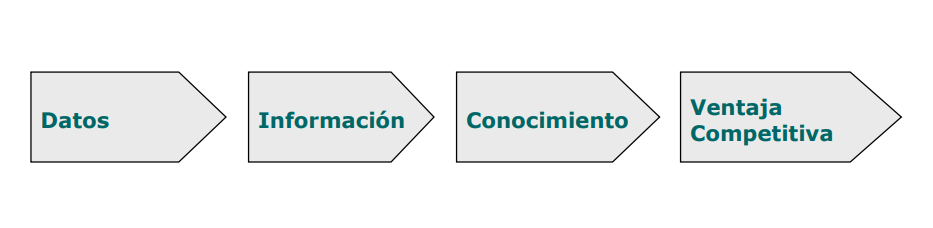
\includegraphics[width=7cm]{./Imagenes/bi} 
\end{center}


\end{itemize}



%----------------------------------------------------------------------------------------
%	DESARROLLO
%----------------------------------------------------------------------------------------

\section{Desarrollo}
%----------------ESTO LO HIZO EL OTRO TEAMMMMMM :v :V -----------------------------------------------------------------------
%----------------ESTO LO HIZO EL OTRO TEAMMMMMM :v :V -----------------------------------------------------------------------
%----------------ESTO LO HIZO EL OTRO TEAMMMMMM :v :V -----------------------------------------------------------------------
%----------------ESTO LO HIZO EL OTRO TEAMMMMMM :v :V -----------------------------------------------------------------------
%----------------HAY QUE CAMBIARLO -----------------------------------------------------------------------
%----------------HAY QUE CAMBIARLO -----------------------------------------------------------------------
%----------------HAY QUE CAMBIARLO -----------------------------------------------------------------------
%----------------HAY QUE CAMBIARLO -----------------------------------------------------------------------

\subsection{¿Que es la inteligencia de negocios?}

La informacion ha propiciado la necesidad de tener mejores, mas rapidos y mas eficientes metodos para extraer y transformar los datos de una organizacion en informacion.
\\ \\
En 1958 \textbf{Hans Peter Luhn}, investigador de la IBM, acuña el termino en el articulo "A Business Intelligence System":
\\ \\
\textsl{''La habilidad de aprender las relaciones de hechos presentados de forma que guien las acciones hacia una meta deseada'' (Hans Luhn, 1958)} \\ \\

 \textbf{ ¿Como funciona el sistema?}

\textsl{''Este sistema de inteligencia utilizará el procesamiento de datos para la auto-abstracción y auto-codificación de documentos y para crear perfiles de interés para cada uno de los "puntos de acción" en una organización.'' (Hans Luhn, 1958)}
\\ \\

En 1989 \textbf{Howard Dresden}, analista de Gartner, propone una definicion formal del concepto.
\\ \\
\textsl{"Conceptos y métodos para mejorar la toma de decisiones comerciales mediante el uso de un sistema de soporte basado en hechos''}
\\ \\
En pocas palabras: \\ \\
\textbf{Es el conjunto de metedologias, aplicaciones, capacidades administrativas de informacion que permite tomar mejores decisiones a los usuarios de una organizacion.}


\subsection{Proceso tradicional de Inteligencia de Negocios}

El proceso de implementación una solución de inteligencia de
negocios tradicional en una organización debe iniciarse por
seleccionar la información relevante para la toma de decisiones,
esto requiere contar con la participación de personal en los niveles
operativo, táctico y gerencial. Se recopilan los datos de las
diferentes fuentes de información existentes (Bases de datos,
archivos, aplicaciones, otros.) ya sean internas o externas con el fin
de normalizarlos, depurarlos y estructurarlos, para almacenarlos
posteriormente en una bodega de datos.

\subsection{¿Qué ventajas nos da usar la inteligencia de negocios?}

- Nos permite tomar decisiones rápidas. \\
- Ayuda a definir escenarios adecuados. \\
- Permite tomar la información, la convierte en conocimiento para la toma de decisiones. \\

\subsection{Beneficions de la inteligencia de negocios}

- Beneficios tangibles, por ejemplo: reducción de costes, generación de ingresos, reducción de tiempos para las distintas actividades del negocio. \\
- Beneficios intangibles: el hecho de que tengamos disponible la información para la toma de decisiones hará que más usuarios utilicen dicha información para tomar decisiones y mejorar la nuestra posición competitiva, por ejemplo: Cuales son los horarios en que más visitan la tienda, cual es el recorrido que hacen en el interior del local. \\
- Beneficios estratégicos: Todos aquellos que nos facilitan la formulación de la estrategia, es decir, a qué clientes, mercados o con qué productos dirigirnos, por ejemplo: ofertas que más solicitan los clientes.

\subsection{Metodología de desarrollo de inteligencia de negocios: Ralph Kimball}
Según los autores (Kimball and Ross, 2002) esta metodología brinda
beneficios para el desarrollo de una Solución de Inteligencia de
Negocios ya que parte por el desarrollo de los Data Marts, para
satisfacer las necesidades específicas de un departamento o área.\\\\
- Planeación y administración del Proyecto\\
- Definición de los Requerimientos del Negocio\\
- Modelado Dimensional\\
- Diseño Físico\\
- Diseño y Desarrollo de la Presentación de Datos\\
- Diseño de la Arquitectura Técnica\\
- Selección de Productos e Instalación\\
- Especificación de Aplicaciones para Usuarios Finales\\
- Desarrollo de Aplicaciones para Usuarios Finales\\
- Implementación\\
- Mantenimiento y crecimiento\\
- Gestión del Proyecto\\

\subsection{Metodología de desarrollo de inteligencia de negocios: Josep Curto}
Según el autor (Curto, 2010) en el libro “Introducción al Business
Intelligence” mencionan que las fases de un proyecto de inteligencia
de negocio son las siguientes:\\\\
-  Análisis y requerimientos\\
- Modelización\\
- Desarrollo\\
- Producción\\
- Formación y Documentación

\subsection{¿Que es el análisis de negocio?}

Es la exploración iterativa y metódica de los datos de una organización, resaltando el análisis estadístico. El análisis empresarial es usado por empresas que toman decisiones basadas en datos. 
\\ \\
Las empresas basadas en datos tratan sus datos como un activo corporativo y buscan convertirlos en una ventaja competitiva. El análisis empresarial depende de la calidad de los datos, de los analistas expertos que entienden las tecnologías y el negocio, y el compromiso de la organización de utilizar los datos para obtener información que ayude en las decisiones comerciales.
\\ \\
Bussiness analytics, se define como el campo del análisis empresarial, se trata del proceso de recopilación, almacenamiento y análisis de datos para asesorar a una empresa mejorando su eficiencia para aumentar sus ingresos.
\\ \\
Si una empresa usa un enfoque que se base en datos en su proceso de toma de decisiones, da como resultado que el análisis juega un rol de gran importancia para la toma de decisiones.  Las personas especialistas en este tema se llaman \textbf{ “Analistas Empresariales”}
\\ \\
Las instituciones recopilan y almacenas datos durante muchos años, pero en los últimos años, han aumentado en cantidad significativa pero la mayor parte de estos datos no están estructurados.  
\\ \\

\textsl{“Según MarTech, el universo digital tiene 2,7 Zettabytes de datos, y si la mayor parte no está estructurada, analizarlo requerirá muchos analistas de datos.  No es de extrañar que el gasto en proyectos de bigdata (proyectos de análisis de negocios) en el 2018 alcanzó los \$114 mil millones de dólares."} (Noodle Staff,2018)

\subsection{Función del análisis de negocio}
Cuando se determina el objetivo comercial del análisis, se selecciona una metodología de análisis y se adquieren datos para respaldar dicho análisis.  Esta adquisición de datos implica la extracción de uno o más sistemas comerciales, la limpieza y la integración en un único almacén de datos.
\\ \\
Este análisis inicial se realiza con una muestra pequeña de datos.  Las herramientas que se utilizan van desde hojas de cálculo, estadística, aplicaciones complejas de extracción de datos y modelado predictivo. A medida que se van descubriendo patrones y relaciones, se hacen nuevas preguntas, completando el proceso analítico, hasta que se cumpla el objetivo comercial.
\\ \\
El despliegue de modelos predictivos implican la puntuación de registros de datos, generalmente en una base de datos, el uso de los puntajes son para optimizar las decisiones en tiempo real, dentro de las aplicaciones y los procesos comerciales del BA, además ayuda en la toma de decisiones tácticas en respuesta a eventos imprevistos.  Y en muchos casos, hasta la toma de decisiones esta automatizada para admitir respuestas en tiempo real.
\subsection{Tipos de análisis de negocio}
Los tipos específicos de análisis de negocios incluyen (Rouse, 2019):


\begin{itemize}	

	\item \textbf{Análisis descriptivo}: Rastrea los indicadores clave de rendimiento (KPI) para comprender el estado actual de un negocio.
	\item \textbf{Análisis predictivo}: Analiza los datos de tendencias para evaluar la probabilidad de resultados futuros.
	\item \textbf{Análisis prescriptivo}: Utiliza el rendimiento pasado para generar recomendaciones sobre cómo manejar situaciones similares en el futuro.

\end{itemize} 

\subsection{Aplicaciones de análisis de negocio}
Las herramientas de análisis de negocio vienen en varias variedades diferentes (Rouse, 2019):
\begin{itemize}	

	\item Herramientas de visualización de datos
	\item Plataformas analíticas de autoservicio
	\item Herramientas de análisis estadístico
	\item Software de informes de inteligencia empresarial
	\item Plataformas de Big Data

\end{itemize} 


%----------------------------------------------------------------------------------------
%	CONCLUSIONES
%----------------------------------------------------------------------------------------

%----------------ESTO LO HIZO EL OTRO TEAMMMMMM :v :V -----------------------------------------------------------------------
%----------------ESTO LO HIZO EL OTRO TEAMMMMMM :v :V -----------------------------------------------------------------------
%----------------ESTO LO HIZO EL OTRO TEAMMMMMM :v :V -----------------------------------------------------------------------
%----------------ESTO LO HIZO EL OTRO TEAMMMMMM :v :V -----------------------------------------------------------------------
%----------------HAY QUE CAMBIARLO -----------------------------------------------------------------------
%----------------HAY QUE CAMBIARLO -----------------------------------------------------------------------
%----------------HAY QUE CAMBIARLO -----------------------------------------------------------------------
%----------------HAY QUE CAMBIARLO -----------------------------------------------------------------------


\section{Conclusiones}
\begin{itemize}	

	\item  En el mundo empresariial, las empresas tienen un area que brinda soporte a los procesos de informacion, estrategia, lo que los lleva a un mercado competitivo, la inteligencia de negocios para una empresa la hace una pieza fundamenta a la hora de tomar mejores deciones.
	\item El numero creciente de pequeñas y medianas empresas da una notoria cifra sobre la ausencia de un sistema de inteligencia empresarial para la gestion de sus empresas. Pero en contraste si tienen conocimiento del concepto y de sus beneficios como el del acceso a datos criticos de la empresa, oportunidades competitivas, tomar mejores deciciones, etc.
	\item Lo que buscan estas herramientas es fomentar la exploración de datos y la toma de decisiones basadas en hechos.
	\item El Business analytics busca prodocir conocimiento estadisticoos y matematicos a partir de datos, con el objetico de generar probales escenarios y opciones con las que lidiar, a comparacion del Business Intelligence que proporciones un analisis a base de datos historicos

\end{itemize} 



%----------------------------------------------------------------------------------------
%	BIBLIOGRAFIA
%----------------------------------------------------------------------------------------


\begin{thebibliography}{99} 

\bibitem[Silvia Chavez y Carmen Contreras, 2018]{}
\newblock Implementación de Business Intelligence, para el proceso de toma de decisiones del área de ventas.

\bibitem[Hans Peter Luhn 1958]{}
\newblock A Business Intelligence System

\bibitem[Alex Rayón, 2015]{Universidad de Deusto}
Conceptos básicos del Business Intelligence.

\bibitem[Jordi Conesa y Josep Curto, 2010]{}
\newblock Introduccion al Business Intelligence

\bibitem[Margaret Rouse, 2019]{}
\newblock Análisis de negocios (BA)

\bibitem[Noodle Editorial Staff, 2018]{}
\newblock Business analytics career paths

\bibitem[Josep Lluis Cano, 2007]{}
\newblock Business Intelligence: competir con información


\bibitem[Curto J., 2010]{} 
\newblock Introducción al Business Intelligence. Editorial UOC.

\bibitem[Kimball R. and Ross M., 2002]{} 
\newblock  The Data Warehouse Toolkit: The Complete Guide to Dimensional Modeling. Wiley
 
\end{thebibliography}


%----------------------------------------------------------------------------------------


\end{document}
